
\documentclass{article}

\newtheorem{example}{Example}
\usepackage{color}
\usepackage{graphicx}
\usepackage{subfig}
\usepackage{url}
\usepackage{relsize}
\renewcommand*{\UrlFont}{\ttfamily\relsize{-1}}
\usepackage{amsmath}

\usepackage{MnSymbol}

\usepackage{float}
\usepackage{wrapfig}
\usepackage{url}
\usepackage{xspace}
\usepackage{anysize}
\usepackage{todonotes}
\usepackage[plain]{algorithm}
\usepackage{multirow}

\usepackage{bm}

\usepackage{algorithm}
\usepackage{algorithmicx}
\usepackage{algpseudocode}

\algtext*{EndIf}


\usepackage{listings}
\usepackage{bold-extra}



\definecolor{dkgreen}{rgb}{0.5,0.5,0.5}
\definecolor{gray}{rgb}{0.5,0.5,0.5}
\definecolor{mauve}{rgb}{0.1,0.5,0.1}
\definecolor{lightgray}{rgb}{0.95,0.95,0.98}
\definecolor{keyw2}{rgb}{0.75,0.1,0.1}
\definecolor{keyw}{rgb}{0,0,0.4}
\lstdefinelanguage{scala}{
  morekeywords={abstract,case,catch,class,def,do,else,extends,false,final,finally,for,if,implicit,import,match,mixin,new,null,object,override,package,private,protected,requires,return,sealed,super,this,throw,trait,true,try,type,val,var,while,with,yield},
  otherkeywords={=>,<-,<\%,<:,>:,\#,@},
  sensitive=true,
  morecomment=[l]{//},
  morecomment=[n]{/*}{*/},
  morestring=[b]",
  morestring=[b]',
  morestring=[b]"""
}

 
\lstset{frame=tb,
  language=scala,
  aboveskip=3mm,
  belowskip=3mm,
  showstringspaces=false,
  columns=flexible,
  basicstyle=\footnotesize\ttfamily,
    keywordstyle=\bfseries\color{keyw},
  backgroundcolor=\color{lightgray},
  numbers=left,
  numbersep=5pt,    
  numberstyle=\small\color{black},
commentstyle=\color{dkgreen},
  stringstyle=\color{mauve},
  frame=single,
  breaklines=true,
  breakatwhitespace=true
  tabsize=3
}

\lstset{language=scala}
\lstset{emph={val, var,def },emphstyle={\color{keyw}\bfseries}}



\papersize{26.7cm}{20.7cm}
\usepackage{tikz}
\definecolor{darkgreen}{rgb}{0,0.66,0} 
\usepackage{pgfplots}
\usetikzlibrary{arrows}

\usepackage{ifthen}
\usepackage{calc}



\date{June 20th, 2014}

\newcommand{\framework}{{\rmfamily\scshape FooPar}\xspace}



\begin{document}



\title{Group Communication Patterns for \\High Performance Computing in Scala}

\author{Felix P. Hargreaves\\ Daniel Merkle \\ Peter Schneider-Kamp\-3ex]
\begin{itemize}
\item Using functional programming concepts, the \emph{Single Program Multiple Data} (SPMD) \cite{spmd} concept can be combined with \emph{Single Instruction Multiple Data (SIMD)} at a data structure level. This allows algorithms to be
formulated in virtually the same way as their serial versions (see Example~\ref{ex:ppi} below).
\item We abstract away peer-to-peer message passing by introducing a set of group communication operations appropriate for HPC use. In this way, we can avoid deadlocks, starvation, race conditions, and other common concurrency issues.
\item We avoid the many pitfalls of manual memory management through the use of a managed programming language running on top of the Java virtual machine. In addition, this provides platform independence.
\end{itemize}

\subsection{Design and Related Work}
While \framework complements the \emph{parallel collections} \cite{odersky11} introduced in Scala
2.8, it is not meant as an extension. This is due to multiple reasons. First,
the parallel collections use workload-splitting strategies leading to communication bottle-necks in distributed memory settings.
Second, they employ an implicit master-slave paradigm unsuitable for massively distributed HPC. Third,
the SPMD paradigm requires launching multiple copies of the process as opposed to branching internally into threads.

\framework differs from other functional programming frameworks for parallel computations in some key aspects. While frameworks like Eden \cite{eden05}, Spark \cite{spark10}, and Scala's own parallel collections \cite{odersky11} try to maximize the level of abstraction, 
this is mostly done through strategies for data-partitioning and distribution which in turn introduce network and computation bottlenecks. Furthermore, these tools lend themselves poorly to parallel runtime analysis hindering 
asymptotic guarantees that might otherwise be achieved. To unaware users, ``automagic'' parallel programming can easily lead to decreased performance due to added overhead and small workloads. With this in mind, 
\framework aims at the sweetspot between high performance computing and highly abstract, maintainable and analyzable programming. This is achieved
by focusing on user-defined workload distribution and deemphasizing fault tolerance. In this way, the performance pitfalls of both \emph{dynamic workload allocation} and the \emph{master-slave} paradigm can be avoided
and \framework can provide HPC parallelism with the conciseness, efficiency and generality expected from mature Scala libraries, while nicely complementing the existing parallel collections of
Scala's standard API for shared memory use.

While Scala's parallel collections are limited to shared memory systems, \framework works both in shared nothing as well as shared memory architectures. Taking some inspiration from MPI~\cite{gabriel04}, \framework implements 
most of the essential operations found in MPI in a more convenient and abstract level as well as expanding upon them. As an example, \framework supports reductions with arbitrary types and variable sizes, e.g. reduction 
by list or string concatenation is entirely possible and convenient in \framework (however inherently unscalable). As an addition, performance impact from the use of concatenation or other size-increasing operations is directly visible through the 
provided asymptotic runtime analysis for operations on the Distributed Memory Parallel Data Structures (cf.\ Section~\ref{sec:dpd}). 

\framework shares goals with the partitioned global address space (PGAS) programming model in the sense that the reference semantics of shared memory systems is combined with the SPMD style of programming. Prominent examples of PGAS are Unified Parallel C, or Co-Array Fortran among others \cite{pgas05}. Focusing on performance and programmability for next-generation architectures, novel languages like X10 and Chapel provide richer execution frameworks and also allow asynchronous creation of tasks \cite{apgas07}. All these languages either resemble and extend existing languages or are designed from scratch; their features are usually accessed via syntactic sugar.
\framework, in contrast, is more oriented towards abstraction by employing distributed data structures and combining this with the mathematical abstraction inherently integrated in functional languages like Scala. This approach 
is somewhat similar to that of STAPL \cite{rauchwerger10}, however, the combination with functional programming has the potential to be more productive and produce more analyzable code.

Finally, comparing to frameworks based on Multiple Program Multiple Data (MPMD), the SPMD paradigm used in \framework emphasizes rank-data mapping, 
where ranks are the IDs of the processing elements in an execution. Section \ref{sec:dpd} shows how
rank-data mappings play a major role in \framework and how it can abstract over serial and parallel programming.

\subsection{Communication Groups}

Instead of explicit message passing, we use the notion of \textit{groups},
a collection of \textit{processes} with a set ofoup
communication operations. We view the instantiation of a DPD of type  as a projection from the set of all processing elements, , defined as .
Subgroup mappings allow for communication algorithms to work independently on a multitude of topologies and sets of processing elements without cluttering the implementations 
with special cases.
Figure \ref{fig:invdoubling} shows a parallel reduction algorithm following the
pattern of the \textit{recursive doubling algorithm} \cite{kumar09}. Here, associativity of the reduction operator is assumed.
This group communication pattern can be directly mapped to the reduction operation
on a DPD as shown in Section~\ref{sec:implementation}. 
Using \framework, complete parallel computations can be described concisely as
a chain of such operations indirectly invoked through operations
on DPDs.\2ex]
\verb!Rank0: ([8.0,16.0]!\\
\verb![24.0,32.0], size = 8,true)!\\
\end{example}

\subsection{Builder/Traversable Pattern}
\label{sec:btp}
For \framework's implementation, a main goal was to avoid
reimplementing the distributed operations such as \texttt{reduceD} and \texttt{mapD}
for each DPD. With the \textit{Builder/Traversable} pattern we achieve this and implement them once and for all,
while maintaining the specific types of the DPDs.

One of the main benefits of Scala's implicits comes from the way the compiler
resolves implicit arguments at compiletime. 
\textit{``If there are several eligible arguments which match the implicit
parameter's type, a most specific one will be chosen using the rules of static
overloading resolution''} \cite{scalref}. Using this feature, type information
can be pushed \textit{upwards} in a type hierarchy via generics and an
adaptation of the \textit{Factory Pattern} \cite{fsttcs2009}, i.e., the
\textit{Builder/Traversable Pattern}, effectively solving the problem depicted in Listing \ref{lst:type}.

\begin{lstlisting}[language=scala]
trait DistTraversable[+T] {
  def elem: Option[T]
  def foreach(f: T => Unit): Unit
  def group: FooParGroup
}
\end{lstlisting}

\noindent The \texttt{DistTraversable} trait presented above
resides at the
base of the type hierarchy (a simplified overview can be seen in
Figure \ref{fig:simplified}).
It defines methods for retrieving a process' local element as well as means of
traversing it. The group is used to supply network communication operations and
follows a DPD through chains of consecutive transformations.

\sloppy{
\framework utilizes Scala's standard library support for the \texttt{Numeric[T]}
type-class \cite{hall1996}.} In combination with the group
communication operations the user gains convenient access to distributed
versions of operations like \texttt{sum, average, min, max} and \texttt{product}
for types \texttt{T}, which provide implicit \texttt{Numeric[T]} values. This
allows user-defined
algebraic types (as well as standard primitives) to work with the built in DPDs in
\framework. The distributed numerical operations are available through
the \texttt{TraversableNumOps} trait.

\begin{figure*}
\centering
\includegraphics[scale=0.27]{traversable.pdf}
\caption{\it Simplified UML diagram of collection package architecture. The
companion objects of \texttt{DistSeq} and \texttt{DistVal} provide type
information to \texttt{DistTraversableLike} through a loose coupling with
implicit definitions of \texttt{CanBuildFrom}.}
\label{fig:simplified}
\end{figure*}

\noindent Both for the type-class support of numeric operations as well as for applying
the \textit{Traversable/Builder} pattern, \framework makes heavy use of
\textit{context bounds}.



In the following we are going to take a look at the implementation of
distributed variables. The implementation of e.g.\ distributed sequences
is analogous except for more complex builders due to the mapping of
indices to ranks.

As shown below \texttt{DistVal[+T]} is basically just the
composition of the traits \texttt{DistTraversableLike} and
\texttt{TraversableNumOps} and thus the most basic implementation of a
DPD.


\begin{lstlisting}[language=scala]
class DistVal[+T]
(val elem: Option[T], val group: FooParGroup)
(implicit val fpapp: FooParApp)
extends DistTraversableLike[T, DistVal[T]]
  with TraversableNumOps[T, DistVal[T]] {
  def size = 1
}
\end{lstlisting}
The real work is performed in \texttt{DistTraversableLike} as well as in the implicit builders of the companion object:
\begin{lstlisting}[language=scala]
object DistVal {
  type DTB[T] = DistTraversableBuilder[T]
  implicit def canBuildFrom[T, U]
  (implicit fpapp: FooParApp): CBF[DistVal[T], U, DistVal[U]] =
    new CBF[DistVal[T], U, DistVal[U]] {
      def apply(): Builder[U, DistVal[U]] = newBuilder(None)
      def apply(from: DistVal[T]): Builder[U, DistVal[U]] =
        newBuilder(Some(from.group))
    } ...
}
\end{lstlisting}

\noindent\sloppy
When the companion objects of an extending class supplies an implicit builder
through the generic trait \texttt{CanBuildFrom[From,Elem,To]}, super classes 
can access this builder at compile-time using explicit self-typing.
The companion object \texttt{DistVal} implements such an implicit definition
of the \texttt{CanBuildFrom} trait.


\sloppy
Finally, the trait \texttt{DistTraversableLike[T,Repr]} defines the collection operations
associated with a distributed traversable by using an implicit builder as a
parameter to the respective methods as seen in the below code.




\begin{lstlisting}[language=scala]
trait DistTraversableLike[+T, +Repr] extends DistTraversable[T] {
  self: Repr =>
  ...
  def reduceD[T1 >: T](assOp: (T1, T1) => T1): Option[T1] = {
    if (group.partOfGroup)
      for (x <- this) group.allOneReduce(x, assOp).foreach(y => return Some(y))
    return None
  }

  def mapD[B, That](f: T => B)(implicit bf: CanBuildFrom[Repr, B, That]): That =
  {
    val b: Builder[B, That] = bf(this)
    if (group.partOfGroup)
      for (x <- this) b += f(x)
    b.result
  } ...
}
\end{lstlisting}
As shown in Figure \ref{fig:simplified}, the same approach is used for
distributed sequences (and other DPDs supported by \framework).





\section{Verification and Testing}
\label{sec:verifytest}

Using core features of functional programming like \textit{higher-order functions} and \textit{immutable data structures}, \framework allows for analyzable and verifiable programs 
to be designed and implemented. Given a higher order function, , which takes a function value parameter, , one can prove the correctness of  given some properties of .
Furthermore, higher order functions can abstract away message passing, including deadlock-safety in their proofs. As an example, \framework provides a distributed method, \texttt{reduceD}, which is proven to be 
correct and deadlock-safe for any associative binary operator, . Once a program can be modeled purely in terms of proven higher-order 
functions, the correctness and safety of that program follows from properties of the function-parameters. In this section, we give a short proof of \textit{All-to-One Reduction} and show 
how specification testing can be used to bridge the gap between proof and practice.
\subsection{Correctness Proof of All-to-One Reduction}

\begin{algorithm}
\caption{\it Functional All-to-One Reduction in \framework.\-5ex]
\begin{algorithmic}
\Function{reduce}{}
\For{\textit{i}  \textbf{until} } 
    \State m 
    \If {} 
      \State \textit{acc}  rcv \Comment{Side-effect}
    \ElsIf {  }
      \State send() \Comment{Side-effect}
    \EndIf
  \EndFor
  
  \If {} 
    \Return Some(value)
  \Else \ \Return None
  \EndIf
\EndFunction
\end{algorithmic}\ \\prod_{r=0}^{2^{n+1}-1}e_r = \left(\prod_{r=0}^{2^n -1}e_r\right) \cdot \left(\prod_{r=2^n}^{2^{n+1}-1}e_r \right)-4ex]

\begin{lstlisting}[label=lst:should,caption=\it Implicit extension with shouldEqual method]
implicit class Should[T](opt: Option[T]) {
  def shouldEqual[U](x: U) = opt.map(_ == x).getOrElse(true)
}
\end{lstlisting}
Listing \ref{lst:should} shows how the method \texttt{shouldEqual} utilizes the \texttt{Option} monad to provide a fallback making sure that processing elements that do not
receive a result always answer \texttt{true} to specification testing.
 


\section{Empirical Results}
\label{sec:empirical}
 
 \begin{figure}[t]
 \centering
 \begin{tikzpicture}[scale=1]
\begin{axis}[
height=6cm,
width=8cm,
legend style={
cells={anchor=east},
at={(0.5,1.2)},anchor=north,
legend plot pos=right
},
xlabel={},
ylabel={seconds},
legend columns=2,
ymax=21, ymin=0,
xmin=100, xmax=600,
grid=major,
symbolic x coords={100,200,300,400,500, 550, 600},
cycle multi list={
{red,mark=square*},
{blue,mark=*}
}]
\addplot coordinates {
(100,0.015295900000000001)
(200,0.0729571)
(300,0.2477926)
(400,0.7547429)
(500,1.504653)
(550,3.7086813999999997)
(600,5.6438586)
};


\addplot coordinates {
(100, 0.0375829)
(200, 0.27488579999999996)
(300, 0.9140756)
(400, 2.7307048000000003)
(500, 5.2165314)
(550, 12.7171593)
(600, 20.0928842)
}; 

\legend{,}

\end{axis}
\end{tikzpicture}
\caption{\it Average walltime in seconds for matrix reduction with multiplication.
\framework with Akka backend and Java with MPJ Express on 16 cores spread across
2 machines.} 
\label{fig:reducetest}
\end{figure}
\framework's ability to reach close-to-optimal performance in real world HPC settings has already been demonstrated extensively for dense matrix-matrix multiplication (cf.\ Figure~\ref{fig:efficiency}) in \cite{ppam13}. Thus, in this section, we focus on two other aspects. First, we compare the performance of a \framework reduction to that of the MPJ Express implementation. Second, we show the framework's ability to scale by presenting 
a parallel implementaiton of the Floyd-Warshall algorithm in \framework and comparing it to a sequential implementation.

\subsection{Comparison to MPJ Express}

We conducted a test of computational scalability reducing  matrices of
varying size with the associative operation of matrix-matrix multiplication. By
varying the size of the matrices we show the performance impact of the
computation part in a reduction in \framework compared to Java+MPJ Express.
Both use the same na\"{\i}ve Java implementation of matrix multiplication utilizing
a 1-dimensional \texttt{double} array matrix representation.



\sloppy
An analysis of the source of MPJ Express reveals an inefficient implementation of the reduce
operation. For matrices of size , it runs in , whereas
\framework \linebreak implements this operation in  . Note that for these running times we assume sufficient bandwidth between
nodes at each stage of the respective algorithms, i.e., they are network
topology oblivious \cite{grama}.

Even when using MPJ Express as a backend,
\framework can still achieve the latter parallel running time because it adds an
algorithmic layer for group communication operations directly above message
passing, thereby diminishing the relevance of backend supplied group
operations. 
Figure \ref{fig:reducetest} shows the expected tendency of running times. Notice
that, even for small sizes of , \framework dominates Java with MPJ Express.

\subsection{Floyd-Warshall Parallelization}
\label{sec:floyd}
The Floyd-Warshall algorithm solves the all-pairs shortest path problem between
all nodes  in a weighted graph. Let  be the weight
of the \textit{minimum-weight path} between  and  among vertices in
the set . The weight of an edge between nod  and  is denoted as .

The dynamic programming formulation can be
expressed as follows, where the shortest path from  to  is given by :\2ex]

\begin{figure}
\begin{center}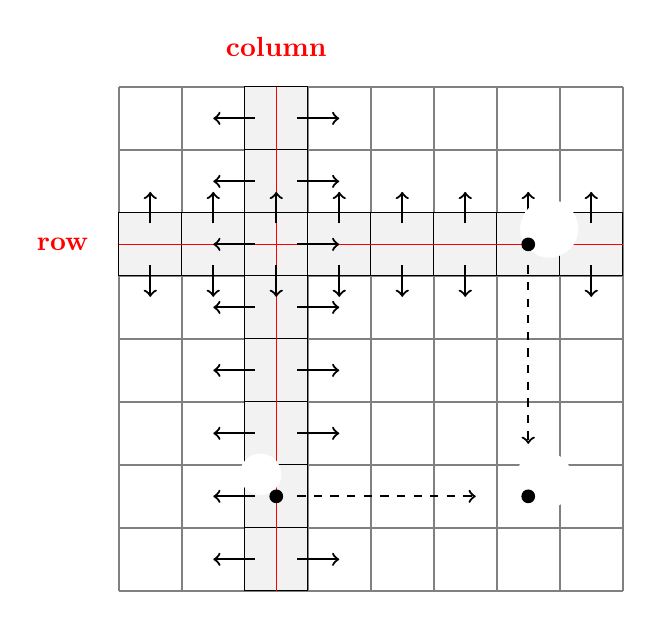
\begin{tikzpicture}[scale=0.8]

\def\n{8}
\def\u{1}
\def\half{\u*0.5}
\def\third{\u/3}
\def\fourth{\u/4}

\def\crossx{2}
\def\crossy{5}

\draw[help lines,thick] (0,0) grid (\n,\n);

\foreach \x in {0,1,...,7} {

	
	\draw [fill=gray!10] (\crossx,\x) rectangle (\crossx+1,\x+1);
	\draw [fill=gray!10] (\x,\crossy) rectangle (\x+1,\crossy+1);

}



\node[above,red,font=\bfseries] at (\crossx+\half,\n+\third) { column};
\draw[-,red,] (\crossx+\half,\n) -- (\crossx+\half,0);

\node[left,red,font=\bfseries] at (0-\third,\crossy+\half) { row};
\draw[-,red] (0,\crossy+\half) -- (\n,\crossy+\half);


\foreach \x in {0,1,...,7} {

	\ifthenelse{\NOT \x = 1}{
	\draw[->,thick] (\crossx+\half+\third,\x+\half) -- (\crossx+1+\half,\x+\half);
	}{};
	\draw[<-,thick] (\crossx-\half,\x+\half) -- (\crossx+\half-\third,\x+\half);
	

	\draw[->,thick] (\x+\half,\crossy+\half+\third) -- (\x+\half,\crossy+1+\third);
	\ifthenelse{\NOT \x = 6}{
	  \draw[->,thick] (\x+\half,\crossy+\half-\third) -- (\x+\half,\crossy-\third);
	}{};
}

\node[fill=white,circle,draw=none,inner sep=0pt,minimum size=21pt] at (6+\half+\fourth,1+\half+\fourth) {};
\draw [fill](6+\half,1+\half)  circle [radius=0.1];

\node[fill=white,circle,draw=none,inner sep=0pt,minimum size=15pt] at (2+\fourth,2-0.15) {};
\draw [fill](2+\half,1+\half)  circle [radius=0.1];

\node[fill=white,circle,draw=none,inner sep=0pt,minimum size=21pt] at (6+\half+\third,5+\half+\fourth) {};
\draw [fill](6+\half,5+\half)  circle [radius=0.1];



\draw[->,thick,dashed]  (\crossx+\half+\third,2-\half) -- (6-\third,2-\half);
\draw[->,thick,dashed]  (6+\half,\crossy+\half-\third) -- (6+\half,2+\third);


\end{tikzpicture}\end{center}
\caption{\it Communication pattern employed in
parallel
Floyd-Warshall:
in iteration , messages of size  are broadcast along  processing elements (in rows and columns).}

\label{fig:floyd}
\end{figure}


\noindent We follow
the parallelization approach from \cite{floyd} (communication pattern presented in Figure \ref{fig:floyd}) and present a scalable version of
the \linebreak parallel Floyd-Warshall algorithm that employs \framework's Distri\-buted Grid (size
, i.e.,  processing elements per dimension):



\begin{lstlisting}[caption=\it Floyd-Warshall implementation in FooPar,label=lst:fw]
def update(row: Vector, col: Vector)(mat: Matrix) = {
  for (i <- 0 until mat.size; j <- 0 until mat(0).size)
    mat(i)(j) = math.min(mat(i)(j), row(j) + col(i))
  mat
}
def floyd(blocks: LazyMatrix, BS: Int) = {
  val dim = blocks.size
  val R = 0 until dim
  val N = dim * BS
  var grid = DistGrid(R, R) mapD { case i :: j :: Nil => blocks(i)(j).data }
  for (k <- 0 until N) {
    val ik = grid.ys.mapD(_(k val kj = grid.xs.mapD(_.map(_(k grid = grid.mapD(update(ik, kj))
  }
  grid
}
\end{lstlisting}


\noindent Briefly explained, Lines 7-10 initialize the 2-dimensional grid and Line 12 is
the inherent sequential loop of the algorithm, which is safely modeled as
a standard for loop. 
Line 13 gets the row  of block  in
the \textit{column} of the calling process.
Similarly, Line 14 gets the column  of the block  in the \textit{row} of the calling process.
Line 15 transforms the grid into the next iteration by updating each block in parallel.

 \begin{figure}[t]
\centering
\begin{tabular}{|l|l||l|l||l|l|}\hline
 \textbf{n} & \textbf{p}& \multicolumn{2}{|c||}{\textbf{Speedup}}& \multicolumn{2}{|c|}{\textbf{Running time in seconds}} \\ & &  MPJ & Akka & MPJ & Akka \\\hline
 \multirow{7}{*}{10080} & 16 &14.65 & 12.76&408.52 &469.06 \\ 
  & 25  &22.56 &19.93&265.3 &300.33 \\ 
  & 36  &26.86&27.40 &222.85 &218.5 \\ 
  & 49  &39.07& 33.81&151.25 &177.05 \\ 
  & 64  &46.17& 36.81&129.66 &162.63 \\ 
  & 81  &56.42&45.07&106.09 &132.83 \\ 
  & 100  &63.54& 60.55&94.21 &98.86 \\ \hline\hline
  \textbf{38000}& \textbf{100} & \textbf{94.28} & 87.39 & 3401.68 & 3669.86 \\ \hline
\end{tabular}

\caption{\it Floyd-Warshall parallel benchmark with input size   and varying numbers of processing elements .
The row for  and  exemplifies speedups on large-scale inputs.} 
\label{fig:floydresults}
\end{figure}
Figure \ref{fig:floydresults} shows scalability result for this implementation. We reach efficiencies of  and  with MPJ-Express and Akka respectively,
i.e., we see that the algorithm is scalable even for large numbers of processing elements. Furthermore, while Akka is mostly dominated by MPJ-Express, the backends behave similarly and the difference in performance 
are likely caused by differences in constants like  or , i.e., startup and per-word transfer times. 

While this example showcases the power of the abstractions in \framework, no work has been done to optimize the computational kernel for the update function (Lines 1-5 of Listing \ref{lst:fw}). We note, however, that 
a highly rewarding aspect of using higher-order functions is that computational kernels are naturally separated from the overall algorithm and, more importantly, completely disconnected from the communication code.

\section{Conclusion}
\label{sec:conclusion}

We have presented \framework, a novel Scala framework for massively parallel distributed memory
computing in Scala, which allows for concise and elegant high-level formulations of
parallel algorithms by abstracting the underlying communication into high-level group
communication operations.

A \framework implementation of the Floyd-Warshall algorithm using distributed grids achieves a near-linear speed-up of
more than 94 on a cluster using 100 processing elements for a matrix of dimension  demonstrating \framework's potential
for expressing scalable algorithms, in this example reducing a computation of nearly 4 days to less than 1 hour.

We have also shown that, independently of the backend, \framework can achieve extremely competitive performance due
to its judicious implementation of the high-level abstractions based on the \textit{Builder/Traversable} pattern.

\subsection{Relation to Previous Work}

\framework was very recently introduced in \cite{ppam13}, wich focuses on parallel algorithms, isoefficiency analysis, and absolute performance. In contrast, in this paper we focus on its architecture and programming model, its implementation in Scala, its comparative performance w.r.t.\ MPJ Express, and its real-world scalability.

\subsection{Future Work}

First, we observe that workload partitioning represents a threshold point of abstraction for parallel programming.
This problem is less pronounced in shared memory architectures, as the partitioning of data can be symbolic. In
distributed memory settings, the communication cost of workload partitioning can easily become a bottleneck of an algorithm.
Furthermore, parallel programs using automated workload partitioning are often harder to analyze.
While automated workload partitioning does not fit directly into \framework,
we plan to explore how \framework can be integrated with a separate dynamic workload allocation module,
in particular for local shared memory workload partitioning in multi-core nodes.

Thirdly, \framework's mix of the SPMD and SIMD paradigms makes it ideal for use in connection with large scale SIMD hardware. CUDA \cite{cuda} and OpenCL \cite{opencl} offer interesting takes on SPMD/SIMD programming,
especially w.r.t. GPU based systems. GPU executions of DPD methods could offer
performance boosts to single-node operations,
in combination with the distributed algorithms already possible in \framework.



\section*{Acknowledgements}

We acknowledge the support by the Danish Council for Independent Research, the Innovation
Center Denmark, the Lawrence Berkeley National Laboratory, and the Scientific Discovery
through Advanced Computing (SciDAC) Outreach Center. 

\vspace{3ex}



\bibliographystyle{plain}

\bibliography{fhpc14}

\end{document}
